\section{Theoretical Analysis and Results}
\subsection{General Considerations}
Without loss of generality, the labels of the nodes in the graph can be selected so that the indices referring to the fake/real news sources appear to be the last ones. Considering $n_p$ as the number of people in the network, $n_s$ as the number of fake and real news sources and $n = n_p + n_s$ the sum thereof, then $A \in \mathbb{R}^{ n \times n}$ can be partitioned as follows:

$$
A = 
\begin{bmatrix}
	\tilde{A}_{n_p \times n_p} & \tilde{B}_{n_p \times n_s} \\
	0_{n_s \times n_p} & I_{n_s \times n_s} \\
\end{bmatrix} 
\quad
$$

Where $\tilde{A}$ describes the reciprocal individual-individual interactions and $\tilde{B}$ describes how people's opinions are directly affected by the sources. The zero and identity matrices below encode the fact that the sources' opinions are not changing over time.\\

The matrix A is row-stochastic, which implies that $1_n$ is eigenvector of A with eigenvalue 1. The Gershgorin disk theorem tells that a row-stochastic matrix cannot have an eigenvalue with magnitude greater than one. By applying the theorem to the treated case, where each diagonal element is different from zero, it can be concluded that the only possible eigenvalue with magnitude equal to 1 is 1 itself. Thus, for each eigenvalue $\mu$ of $A$, $\mu=1$ or $|\mu|<1$.


%%% old version
%The following therefore holds for the spectrum of A:
%\begin{align*}
%spec(A) \subset \{\mu \in \mathbb{C}^n,\ \mu_i = 1\ \forall i & \in \{1,..,n_{mult}\},\\
%| \mu_i | < 1 \text{ otherwise}\}
%\end{align*}
%%% old version 
%%%%% work in progress
%where $n_{mult}$ is the algebraic multiplicity of 1.

%%%%%
Denoting $\rho(A)$ the spectral radius, we have $\rho(A) = 1$, thus the matrix A cannot be stable but it is semi-stable if and only if the eigenvalue $1$ is semi-simple.

The randomness in the graph generation process does not allow to conclude much more deterministically. However, the properties of $\tilde{A}$ are of great importance to infer the system behavior.
For the numerical experiments in
Sections~\ref{sec:Instr_Level} to~\ref{sec:manipulability}, the model parameters were set to $n_p = 100$, $C$ = 0.2, nRoot = 4 and news connection type \textit{local}. It is remarkable that with the proposed set up $\tilde{A}$ describes a strongly-connected graph in 99.4$\%$ of the cases. This value was obtained after generating 10000 different networks.
%The parameters $n_p$, $C$, nRoot and the news connection type, fully describe the probabilistic model to generate connections between a person and its neighbors, see Subsection~\ref{subsec:connections_existence}.
 The graph is directed and a connection from node $i$ to node $j$ implies a connection from $j$ to $i$ but with different weights in general. The 0.6$\%$ represents therefore some pathological and unlikely cases where part of the network is completely disconnected from the rest. This could represent an isolated and separated society living in our simulated world. Since these cases are not relevant for the aim of this project (the news spread in a connected society is studied), these cases were simply discarded. From now on, it can therefore be assumed that the graph describing the individual-individual interactions is strongly connected, meaning that the matrix $\tilde{A}$ is irreducible.\newline In the following, the steady state behavior of the discrete time averaging system of Equation~\eqref{eq:model}
is analyzed under various conditions.

\subsection{$n_s = 0$}
If there are no sources, the matrix A = $\tilde{A}$ describes a strongly connected digraph. Each node has a self-cycle meaning that the single strongly connected component is aperiodic. The graph is therefore strongly connected and aperiodic, which implies that the matrix A describing it is primitive. This, together with the fact that A is row-stochastic, implies that A is semi-convergent and that the discrete-time averaging system convergences to consensus and namely to:
$$
x_{\infty} = (w^Tx(0))1_n = \left(\sum_{i=1}^{n}w_ix_i(0)\right)1_n
$$
$$
w^TA = w^T,\ 
Av = v,\ 
v \geq 0,\ w \geq 0,\ w^Tv = 1
$$
\subsection{$n_s \geq 2$}
\begin{figure}[!t]
	\centering
	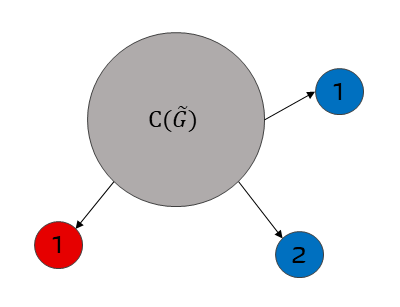
\includegraphics[width=2.5in]{Figures/condensation_digraph.png}
	\caption{Example of a network condensation of digraph $G$. All individuals belong to a single strongly connected component $C(\tilde{G})$ (grey), there are one source of fake news (red) and two sources of real news (blue). $G$ is the digraph associated to the adjacency matrix $A$, $\tilde{G}$ is associated to $\tilde{A}$.}
	\label{pics:condensation_digraph_example}
\end{figure}
Figure~\ref{pics:condensation_digraph_example} shows an example condensation digraph for a network with irreducible $\tilde{A}$, one source of fake news and two sources of real news. The condensation is in general composed of $n_s+1$ nodes.  The news sources are all represented by sinks and the network of people by a single node connected to all sinks. \newline
All strongly connected components are furthermore aperiodic: both the sources and the individuals have self-loops.
According to theorem 5.2 from the lecture notes, for a row-stochastic matrix A with multiple aperiodic sinks ($n_s \geq 2$), the following holds:
\begin{enumerate}
	\item
	A is semi-convergent.
	\item
	The eigenvalue 1 is semi-simple with multiplicity $n_s$ and all other eigenvalues $|\mu|<1$.
	\item
	The left eigenvectors $w^q \in \mathbb{R}^n$, $q\in \{1,...,n_s\}$, of A corresponding to the eigenvalue 1 can be selected to satisfy: $w^q\geq0,\ 1_n^Tw^q=1$, $w^q_i>0$ if and only if node i belongs to sink q.
	\item
	$
	x_{\infty}^i = 
	\begin{cases}
	(w^q)^Tx(0),& \text{node i $\in$ sink q}\\
	\sum_{q=1}^{n_s} z_{i,q}((w^q)^Tx(0)), & \text{otherwise}
	\end{cases}
	$
	where $z_{i,q},\ q\in\{1,...,n_s\}$, are convex combination coefficients and $z_{i,q} > 0$ if and only if there exists a directed path from node i to the sink q. This is always true for the individuals in this case making $z_{i,q} > 0\ \forall\ q \in \{1,...,n_s\}$ and $i \in \{1,...,n_p\}$.
\end{enumerate}
The third statement for the treated scenario implies $(w^q)^T = (0_{1 \times n_p},\ 0_{1 \times (q-1)},\ 1,\ 0_{1 \times (n_s-q)})$. This is because there is only one node in each sink q. The index referring to that node is therefore the only one different from zero in $w^q$. $1_n^Tw=1$ enforces then its value to be exactly equal to 1. By plugging this result into iv), one can obtain the following:
$$
x_{\infty}^i = 
\begin{cases}
	x(0)^{n_p+q},& \text{node i $\in$ sink q}\\
	\sum_{q=1}^{n_s} z_{i,q}(x(0)^{n_p+q}), & \text{otherwise}
\end{cases}
$$
where $x(0)^{n_p+q}$ is the $(n_p+q)^{th}$ element of x(0) (= the $q^{th}$ source initial condition). Therefore, the steady state value of $x$ does not depend on the population initial conditions. It just depends on the sources. Furthermore, it depends on $z_{i,q}$, whose value is strictly greater than zero for the population as  illustrated earlier. Their exact value depends on the random variables in our model, thus it cannot be estimated in general and their expected values depend on the traits and the connections model. \newline
The result can be further simplified by plugging in the values of the initial conditions (-1 for fake and +1 for real news sources):
$$
x_{\infty}^i = 
\begin{cases}
\delta_q,& \text{node i $\in$ sink q}\\
\sum_{q=1}^{n_s} z_{i,q}\delta_q, & \text{otherwise}
\end{cases}
$$

$$ \text{where }
\delta_q = 
\begin{cases}
1,& \text{sink q is real news source}\\
-1,& \text{sink q is fake news source}
\end{cases}
$$


The parameters $z_{i,q},\ q\in\{1,...,n_s\}$, are convex combination coefficients, which means that $\sum_{q=1}^{n_s} z_{i,q} = 1$ $\forall$ i.
If there is only one type of sources (either fake or real news), then $\sum_{q=1}^{n_s} z_{i,q}\delta = \delta*\sum_{q=1}^{n_s} z_{i,q} = \delta$ which is either +1 or -1 depending on whether the only type of source is real or fake: 
$x_\infty = 
\begin{cases}
1_n,& \text{Only real news sources}\\
-1_n,& \text{Only fake news sources}
\end{cases}$
\\This is consistent with the expectations: if there is only one type of news sources, the entire population will tend to fully believe this source as time goes to infinity. This is independent of the population initial condition.
\subsection{$n_s = 1$}
If $n_s=1$, then there is either a single fake or a single real news source. The condensation digraph contains a single aperiodic sink, which is composed by the news source itself. The news source is reachable from every node in G and the other nodes are reachable from every node in the graph but from the source. This makes the news source the only globally reachable node in the graph. Its subgraph is furthermore aperiodic because of the self-loops. From this, it follows for the row-stochastic matrix A:
\begin{enumerate}
	\item
	The eigenvalue 1 is simple and all other eigenvalues $\mu$ satisfy $|\mu|<1$
	\item
	A is semi-convergent and $lim_{k->\infty} A^k = 1_n w^T$, where $w \in \mathbb{R}^n$ satisfies $w\geq0, 1_n^T w = 1$, and $w^TA=w^T$
	\item
	$w\geq0$ is the left dominant eigenvector of A and $w_i>0$ if and only if $i$ is globally reachable. As previously discussed, this is the case only for the source in the considered scenario. \newline
	$\implies$ $w^T = (0,...,0,1)$.
	\item
	$$x_\infty = (w^T x(0))1_n = x(0)_{n_p+1} 1_n=$$
	$$= \begin{cases}
	1_n,& \text{Real news source}\\
	-1_n & \text{Fake news source}
	\end{cases}$$
	Where $x(0)_{n_p}$ is the $n_p^{th}$ element of $x(0)$ (the source initial condition). 
\end{enumerate}
Therefore, in the case with only one news source, the whole network converges to the source opinion as time goes to infinity and this is independent of the population initial condition.



\subsection{Population network not strongly connected}
\begin{figure}[!t]
	\centering
	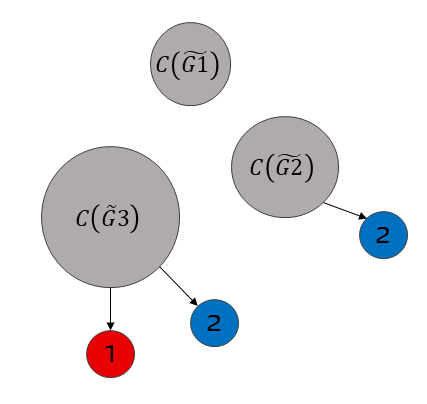
\includegraphics[width=2.5in]{Figures/not_strongly_connected.png}
	\caption{Example of a not fully connected network condensation digraph. The people interactions are summarized by the respective subnetworks. There are one source of fake news (red) and two sources of real news (blue).}
	\label{pics:nonconnectednetwork}
\end{figure}
As previously discussed, if the population network is not strongly connected, there are two or more separated population networks, which are strongly connected if taken individually. Figure~\ref{pics:nonconnectednetwork} shows the condensation digraph for an example of a disconnected network. Each sub-network might have one or more nodes and forms a strongly connected network. Each sub-network might or might not be connected to one or multiple sources. \newline
In order to find the steady state, each network can be observed separately:
\begin{itemize}
	\item 
	Provide a different label to each sub-network, $\tilde{G}_i$, $i \in \mathbb{N}$
	\item 
	For every sub-network $i$,
	\begin{itemize}
		\item 
		Count the number of nodes corresponding to individuals $n_p^i$ and the number of news sources $n_s^i$ connected to $\tilde{G}_i$. 
		\item 
		Apply the formulas presented in the previous sections to find the steady state of the sub-network $i$.
	\end{itemize}
\end{itemize}
The sub-network steady states are therefore independent of each other. The results will be therefore completely different in general. 